\documentclass{article}
\usepackage{amsmath}
\usepackage{amsfonts}
\usepackage{graphicx}
\usepackage[utf8x]{inputenc}
\usepackage{listings}
\usepackage{color} %red, green, blue, yellow, cyan, magenta, black, white
\usepackage[sfdefault]{roboto}  %% Option 'sfdefault' only if the base font of the document is to be sans serif
\usepackage[T1]{fontenc}
\definecolor{codegreen}{rgb}{0,0.6,0}
\definecolor{codegray}{rgb}{0.5,0.5,0.5}
\definecolor{codepurple}{rgb}{0.58,0,0.82}
\definecolor{backcolour}{rgb}{0.95,0.95,0.92}

\title{Machine Learning lecture notes}
\author{Khoa Hoang Viet \thanks{based on Andrew Ng's Machine Learning course in coursera.org}}
\date{\today}
\begin{document}

\lstdefinestyle{mystyle}{
    backgroundcolor=\color{backcolour},
    commentstyle=\color{codegreen},
    keywordstyle=\color{magenta},
    numberstyle=\tiny\color{codegray},
    stringstyle=\color{codepurple},
    basicstyle=\footnotesize,
    breakatwhitespace=false,
    breaklines=true,
    captionpos=b,
    keepspaces=true,
    numbers=left,
    numbersep=5pt,
    showspaces=false,
    showstringspaces=false,
    showtabs=false,
    tabsize=2
}

\lstset{style=mystyle}

\section{Cost Function and Backpropagation}
\subsection{Cost Function}
Let's first define a few variables that we will need to use:
\begin{itemize}
  	\item L = total number of layers in the network
  	\item $s_j$ number of units (not counting bias unit) in layer l
  	\item K = number of output units/classes
\end{itemize}

Recall that in neural networks, we may have many output nodes. We denote $h_\Theta(x)_k$  as being a hypothesis that results in the $k^{th}$ output. Our cost function for neural networks is going to be a generalization of the one we used for logistic regression.
\begin{gather*}
	J(\Theta) = - \frac{1}{m} \sum_{i=1}^m \sum_{k=1}^K \left[y^{(i)}_k \log ((h_\Theta (x^{(i)}))_k) + (1 - y^{(i)}_k)\log (1 - (h_\Theta(x^{(i)}))_k)\right] \\
	+ \frac{\lambda}{2m}\sum_{l=1}^{L-1} \sum_{i=1}^{s_l} \sum_{j=1}^{s_{l+1}} ( \Theta_{j,i}^{(l)})^2
\end{gather*}

We have added a few nested summations to account for our multiple output nodes. In the first part of the equation, before the square brackets, we have an additional nested summation that loops through the number of output nodes.

In the regularization part, after the square brackets, we must account for multiple theta matrices. The number of columns in our current theta matrix is equal to the number of nodes in our current layer (including the bias unit). The number of rows in our current theta matrix is equal to the number of nodes in the next layer (excluding the bias unit). As before with logistic regression, we square every term.

Note:
\begin{itemize}
	\item the double sum simply adds up the logistic regression costs calculated for each cell in the output layer
	\item the triple sum simply adds up the squares of all the individual $\Theta$s in the entire network
	\item the i in the triple sum does not refer to training example i
\end{itemize}

\subsection{Backpropagation Algorithm}
"Backpropagation" is neural-network terminology for \textbf{minimizing our cost function}, just like what we were doing with gradient descent in logistic and linear regression. Our goal is to compute:
$$\min_\Theta J(\Theta)$$

That is, we want to minimize our cost function J using an optimal set of parameters in theta. In this section we'll look at the equations we use to compute the partial derivative of $J(\Theta)$:
$$\dfrac{\partial}{\partial \Theta_{i,j}^{(l)}}J(\Theta)$$

To do so, we use the following algorithm:\\
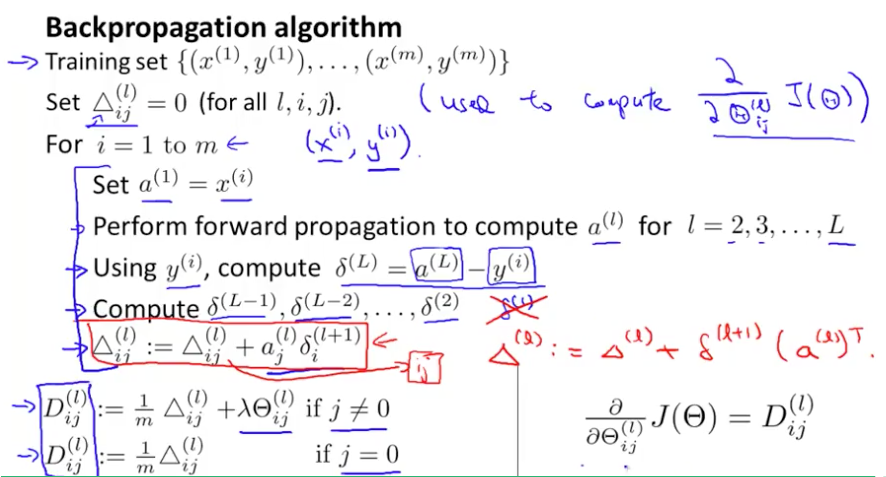
\includegraphics[width=\textwidth]{Backpropagation_Algorithm.png}

\noindent\textbf{Back propagation Algorithm}

Given training set $\lbrace (x^{(1)}, y^{(1)}) \cdots (x^{(m)}, y^{(m)})\rbrace$

Set $\Delta^{(l)}_{i,j} := 0$ for all (l,i,j), (hence you end up having a matrix full of zeros)

For training example t =1 to m:
\begin{enumerate}
	\item \textbf{Set $a^{(1)} := x^{(t)}$}
	\item \textbf{Perform forward propagation to compute $a^{(l)}$ for l=2,3,…,L}\\
	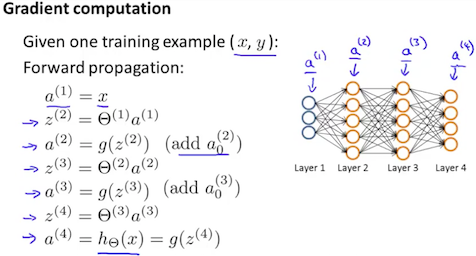
\includegraphics[scale=0.65]{Forward_propagation.png}
	\item \textbf{Using $y^{(t)}$, compute $\delta^{(L)} = a^{(L)} - y^{(t)}$}

	Where L is our total number of layers and $a^{(l)}$ is the vector of outputs of the activation units for the last layer. So our "error values" for the last layer are simply the differences of our actual results in the last layer and the correct outputs in y.
	\item \textbf{Compute $\delta^{(L-1)}, \delta^{(L-2)},\dots,\delta^{(2)}$ using $$\delta^{(l)} = ((\Theta^{(l)})^T \delta^{(l+1)})\ .*\ a^{(l)}\ .*\ (1 - a^{(l)})$$}

	The delta values of layer l are calculated by multiplying the delta values in the next layer with the theta matrix of layer l. We then element-wise multiply that with a function called g', or g-prime, which is the derivative of the activation function g evaluated with the input values given by $z^{(l)}$.

	The g-prime derivative terms can also be written out as:
	$$g'(z^{(l)}) = a^{(l)}\ .*\ (1 - a^{(l)})$$
	\item \textbf{$\Delta^{(l)}_{i,j} := \Delta^{(l)}_{i,j} + a_j^{(l)} \delta_i^{(l+1)}$ or $\Delta^{(l)} := \Delta^{(l)} + \delta^{(l+1)}(a^{(l)})^T$}

	Hence we update our new $Delta$ matrix.
	$$D^{(l)}_{i,j} := \dfrac{1}{m}\left(\Delta^{(l)}_{i,j} + \lambda\Theta^{(l)}_{i,j}\right)$$
	$$D^{(l)}_{i,j} := \dfrac{1}{m}\Delta^{(l)}_{i,j}$$
	The capital-delta matrix D is used as an "accumulator" to add up our values as we go along and eventually compute our partial derivative. Thus we get $$\frac \partial {\partial \Theta_{ij}^{(l)}} J(\Theta) = D_{ij}^{(l)}$$

\end{enumerate}

\subsection{Backpropagation Intuition}
The cost function is:
\begin{gather*}
	J(\theta) = - \frac{1}{m} \sum_{t=1}^m\sum_{k=1}^K  \left[ y^{(t)}_k \ \log (h_\theta (x^{(t)}))_k + (1 - y^{(t)}_k)\ \log (1 - h_\theta(x^{(t)})_k)\right] \\
	+ \frac{\lambda}{2m}\sum_{l=1}^{L-1} \sum_{i=1}^{s_l} \sum_{j=1}^{s_l+1} ( \theta_{j,i}^{(l)})^2
\end{gather*}

If we consider simple non-multiclass classification (k = 1) and disregard regularization, the cost is computed with:
$$cost(t) =y^{(t)} \ \log (h_\theta (x^{(t)})) + (1 - y^{(t)})\ \log (1 - h_\theta(x^{(t)}))$$

More intuitively you can think of that equation roughly as:
$$cost(t) \approx (h_\theta(x^{(t)})-y^{(t)})^2$$

Intuitively, $\delta_j^{(l)}$ is the "error" for $a^{(l)}_j$ (unit j in layer l)

More formally, the delta values are actually the derivative of the cost function:
$$\delta_j^{(l)} = \dfrac{\partial}{\partial z_j^{(l)}} cost(t)$$

Recall that our derivative is the slope of a line tangent to the cost function, so the steeper the slope the more incorrect we are.

Note: In lecture, sometimes i is used to index a training example. Sometimes it is used to index a unit in a layer. In the Back Propagation Algorithm described here, t is used to index a training example rather than overloading the use of i.

\section{Backpropagation in Practice}
\subsection{Implementation Note: Unrolling Parameters}
With neural networks, we are working with sets of matrices:
\begin{align*}
	\Theta^{(1)}, \Theta^{(2)}, \Theta^{(3)}, \dots \\
	D^{(1)}, D^{(2)}, D^{(3)}, \dots
\end{align*}

In order to use optimizing functions such as "fminunc()", we will want to "unroll" all the elements and put them into one long vector:

\begin{lstlisting}[language=Octave]
thetaVector = [Theta1(:); Theta2(:); Theta3(:);]
deltaVector = [D1(:); D2(:); D3(:)]
\end{lstlisting}

If the dimensions of Theta1 is 10x11, Theta2 is 10x11 and Theta3 is 1x11, then we can get back our original matrices from the "unrolled" versions as follows:

\begin{lstlisting}[language=Octave]
Theta1 = reshape(thetaVector(1:110),10,11)
Theta2 = reshape(thetaVector(111:220),10,11)
Theta3 = reshape(thetaVector(221:231),1,11)
\end{lstlisting}

\subsection{Gradient Checking}
Gradient checking will assure that our backpropagation works as intended.

We can approximate the derivative of our cost function with:
$$\dfrac{\partial}{\partial\Theta}J(\Theta) \approx \dfrac{J(\Theta + \epsilon) - J(\Theta - \epsilon)}{2\epsilon}$$

With multiple theta matrices, we can approximate the derivative with respect to $\Theta_j$ as follows:
$$\dfrac{\partial}{\partial\Theta_j}J(\Theta) \approx \dfrac{J(\Theta_1, \dots, \Theta_j + \epsilon, \dots, \Theta_n) - J(\Theta_1, \dots, \Theta_j - \epsilon, \dots, \Theta_n)}{2\epsilon}$$

A good small value for ${\epsilon}$ (epsilon), guarantees the math above to become true. If the value be much smaller, may we will end up with numerical problems. The professor Andrew usually uses the value ${\epsilon = 10^{-4}}$.

We are only adding or subtracting epsilon to the $Theta_j$ matrix. In octave we can do it as follows:

\begin{lstlisting}[language=Octave]
epsilon = 1e-4;
for i = 1:n,
  thetaPlus = theta;
  thetaPlus(i) += epsilon;
  thetaMinus = theta;
  thetaMinus(i) -= epsilon;
  gradApprox(i) = (J(thetaPlus) - J(thetaMinus))/(2*epsilon)
end;
\end{lstlisting}

We then want to check that gradApprox ≈ deltaVector.

Once you've verified once that your backpropagation algorithm is correct, then you don't need to compute gradApprox again. The code to compute gradApprox is very slow.

\subsection{Random Initialization}
Initializing all theta weights to zero does not work with neural networks. When we backpropagate, all nodes will update to the same value repeatedly.

Instead we can randomly initialize our weights:

Initialize each $\Theta^{(l)}_{ij}$ to a random value between $[-\epsilon,\epsilon]$:
$$\epsilon = \dfrac{\sqrt{6}}{\sqrt{\mathrm{Loutput} + \mathrm{Linput}}}$$
$$\Theta^{(l)} =  2 \epsilon \; \mathrm{rand}(\mathrm{Loutput}, \mathrm{Linput} + 1)    - \epsilon$$

\begin{lstlisting}[language=Octave]
If the dimensions of Theta1 is 10x11, Theta2 is 10x11 and Theta3 is 1x11.

Theta1 = rand(10,11) * (2 * INIT_EPSILON) - INIT_EPSILON;
Theta2 = rand(10,11) * (2 * INIT_EPSILON) - INIT_EPSILON;
Theta3 = rand(1,11) * (2 * INIT_EPSILON) - INIT_EPSILON;
\end{lstlisting}

rand(x,y) will initialize a matrix of random real numbers between 0 and 1. (Note: this epsilon is unrelated to the epsilon from Gradient Checking)

\subsection{Putting it Together}
First, pick a network architecture; choose the layout of your neural network, including how many hidden units in each layer and how many layers total.
\begin{itemize}
	\item Number of input units = dimension of features $x^{(i)}$
	\item Number of output units = number of classes
	\item Number of hidden units per layer = usually more the better (must balance with cost of computation as it increases with more hidden units)
	\item Defaults: 1 hidden layer. If more than 1 hidden layer, then the same number of units in every hidden layer.
\end{itemize}

\textbf{Training a Neural Network}

\begin{enumerate}
	\item Randomly initialize the weights
	\item Implement forward propagation to get $h_\theta(x^{(i)})$
	\item Implement the cost function
	\item Implement backpropagation to compute partial derivatives
	\item Use gradient checking to confirm that your backpropagation works. Then disable gradient checking.
	\item Use gradient descent or a built-in optimization function to minimize the cost function with the weights in theta.
\end{enumerate}

When we perform forward and back propagation, we loop on every training example:

\begin{lstlisting}[language=Octave]
for i = 1:m,
	Perform forward propagation and backpropagation using example (x(i),y(i))
	(Get activations a(l) and delta terms d(l) for l = 2,...,L
\end{lstlisting}
\end{document}
